\documentclass[a4paper,10pt]{article}

\usepackage[utf8x]{inputenc}
\usepackage{makeidx}
\usepackage{listings}
\usepackage{color}
\usepackage{graphicx}
\usepackage{hyperref}

%\usepackage{html}   %  *always* load this for LaTeX2HTML
%\begin{htmlonly}
%  \usepackage{verbatim}
%  \providecommand{\lstlisting}[2][]{\verbatiminput{#2}}
%\end{htmlonly}

\input colordvi
\definecolor{lightblue}{rgb}{.3,.5,1}
\definecolor{orange}{rgb}{1,.7,0}
\definecolor{darkorange}{rgb}{1,.4,0}
\definecolor{darkgreen}{rgb}{0,.4,0}
\definecolor{darkblue}{rgb}{0,0,.4}
\definecolor{darkred}{rgb}{.56,0,0}
\definecolor{gray}{rgb}{.3,.3,.3}
\definecolor{darkgray}{rgb}{.2,.2,.2}
\definecolor{shadecolor}{gray}{0.925}

\lstdefinelanguage{GEXF}{
    morekeywords=[0]{gexf, meta, graph, creator, description, nodes, edges, node, edge, attributes, attribute, options, attvalues, attvalue, default, keywords, color, size, position, shape, thickness, parents, parent, spells, spell, viz},
    morekeywords=[1]{id, for, pid, label, source, target, mode, defaultedgetype, type, lastmodifieddate, start, startopen, end, endopen, timetype, cardinal, class, count, title, value, r, g, b, x, y, z, a, xmlns},
    morekeywords=[2]{simple, double, static, dynamic, integer, double, float, boolean, liststring, string, date, anyURI},
    morestring=[b]",
}

\lstdefinestyle{gexf}{
    language=GEXF,
    xleftmargin=\parindent,
    xrightmargin=\parindent,
    aboveskip=3mm,
    belowskip=3mm,
    tabsize=2,
    columns=[l]fullflexible,
    showstringspaces=false,
    % text styles
    basicstyle=\scriptsize\ttfamily,
    commentstyle=\footnotesize\rmfamily\em,
    stringstyle=\rmfamily\em\color{gray},
    keywordstyle=[0]\color{blue},
    keywordstyle=[1]\color{darkorange},
    keywordstyle=[2]\underbar,
    % numbers
    numbers=left,
    numberstyle=\tiny,
    stepnumber=3,
    firstnumber=1,
    % decoration
    frame=shadowbox,
    frameround=tttf
    %backgroundcolor=\color{shadecolor}
}

\lstdefinelanguage{RNC}{
    morekeywords=[1]{start,element,attribute,text,empty,string,text},
    morekeywords=[2]{default,namespace,datatypes},
    morekeywords=[3]{grammar,include,parent,inherit},
    morekeywords=[4]{xsd},
    morekeywords=[5]{defaultValue},
    morestring=[b]",
    morecomment=[l]{\#},
    alsodigit={-},
    sensitive
}


\lstdefinestyle{rnc}{
    language=RNC,
    basicstyle=\scriptsize\ttfamily,
    commentstyle=\footnotesize\sffamily\em\color{darkgreen},
    stringstyle=\sffamily\color{red},
    keywordstyle=[1]\color{blue}\bfseries,
    keywordstyle=[2]\color{lightblue}\bfseries,
    keywordstyle=[3]\color{lightblue}\bfseries,
    keywordstyle=[4]\color{darkgreen}\bfseries,
    keywordstyle=[5]\color{orange}\bfseries
}

%\lstdefinestyle{xml}{
    language=XML,
    xleftmargin=\parindent,
    xrightmargin=\parindent,
    aboveskip=3mm,
    belowskip=3mm,
    basicstyle=\footnotesize\ttfamily,
    commentstyle=\small\rmfamily\em,
    tabsize=2,
    columns=[l]fullflexible,
    showstringspaces=false,
    % keywords
    keywordstyle=\color{blue}\bfseries,
    stringstyle=\color{red},
    usekeywordsintag=false,
    markfirstintag=true,
    % numbers
    numbers=left,
    numberstyle=\tiny,
    stepnumber=3,
    firstnumber=1,
    % decoration
    frame=shadowbox,
    frameround=tttf,
    backgroundcolor=\color{shadecolor}
}


\hypersetup{
    bookmarks=true,         % show bookmarks bar?
    unicode=false,          % non-Latin characters in Acrobat’s bookmarks
    pdftoolbar=true,        % show Acrobat’s toolbar?
    pdfmenubar=true,        % show Acrobat’s menu?
    pdffitwindow=false,     % window fit to page when opened
    pdfstartview={FitH},    % fits the width of the page to the window
    pdftitle={GEXF 1.3 Primer},    % title
    pdfauthor={GEXF Working Group},     % author
    pdfsubject={GEXF 1.3 Primer},   % subject of the document
    pdfcreator={GEXF Working Group},   % creator of the document
    pdfproducer={GEXF Working Group}, % producer of the document
    pdfkeywords={gephi gexf graph}, % list of keywords
    pdfnewwindow=true,      % links in new window
    colorlinks=false,       % false: boxed links; true: colored links
    linkcolor=red,          % color of internal links
    citecolor=green,        % color of links to bibliography
    filecolor=magenta,      % color of file links
    urlcolor=cyan           % color of external links
}

\makeindex


%opening
\title{GEXF 1.3.1 Primer}
\author{GEXF Working Group}

\begin{document}

\maketitle

\begin{abstract}
GEXF Primer is a non-normative document intended to provide an easily readable description of the GEXF facilities, and is oriented towards quickly understanding how to create GEXF documents. This primer describes the language features through examples which are complemented by references to normative texts. Specification is in \href{http://relaxng.org/compact-tutorial-20030326.html}{RelaxNG Compact} grammar.
\end{abstract}

\tableofcontents

\section{Introduction} \label{introduction}

\paragraph{}
This document, GEXF Primer, provides an description of GEXF, and should be used alongside the formal descriptions of the language contained in the GEXF specification. The intended audience of this document includes application developers whose programs read and write GEXF files, and users who want to communicate with programs using GEXF import/export. The text assumes that you have a basic understanding of XML 1.0 and  XML-Namespaces. Basic knowledge of XML Schema is also assumed for some parts of this document. Each major section of the primer introduces new features of the language, and describes those features in the context of concrete examples.

\paragraph{}
Section 2 covers the basic mechanisms of GEXF. It describes how to declare a simple graph by defining its nodes and edges and how to add simple user data to the graph.

\paragraph{}
Section 5 describes dynamic graph model (i.e. graphs over time).

\paragraph{}
Section 6 describes mechanisms for extending GEXF to add specific data with the Visualization module in example.

\paragraph{}
The primer is a non-normative document, which means that it does not provide a definitive specification of the GEXF language. The examples and other explanatory material in this document are provided to help you understand GEXF, but they may not always provide definitive answers. In such cases, you will need to refer to the GEXF specification, and to help you do this, we provide many links pointing to the relevant parts of the specification.

\paragraph{}
In this document, we may use the terms network and graph interchangeably.

\section{Basic Concepts} \label{basic}

The purpose of a GEXF document is to define a graph representing a network. Let us start by considering the minimal graph shown in the figure below. It contains 2 nodes and 1 edge.

\begin{figure}[!ht]
  \begin{center}
  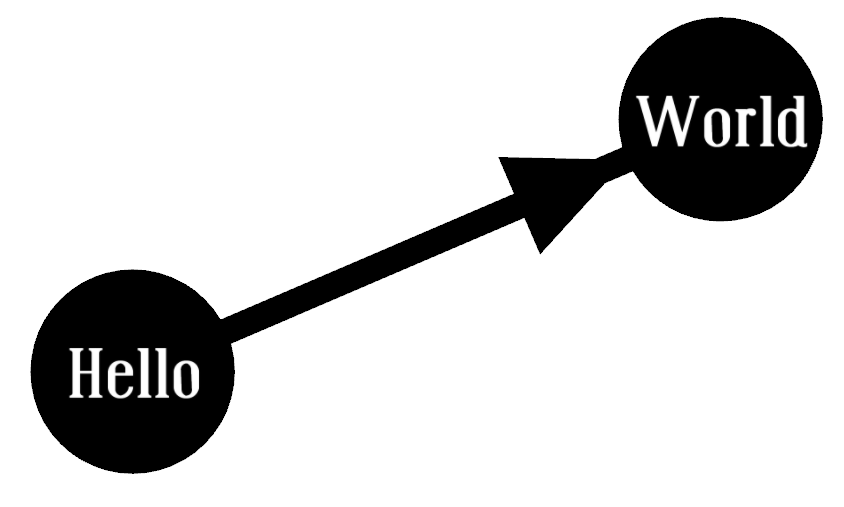
\includegraphics[scale=0.15]{res/simple.png}
  \caption{Hello-world graph}
  \end{center}
\end{figure}

\subsection{A Simple Graph}

This is a dummy graph:

\lstset{ style=gexf }
\begin{lstlisting}[caption={Hello world!},label=helloworld]
<?xml version="1.0" encoding="UTF-8"?>
<gexf xmlns="http://gexf.net/1.3.1"
       xmlns:xsi="http://www.w3.org/2001/XMLSchema-instance"
       xsi:schemaLocation="http://gexf.net/1.3.1
                             http://gexf.net/1.3.1/gexf.xsd"
      version="1.3">
  <meta lastmodifieddate="2009-03-20">
    <creator>Gephi.org</creator>
    <title>Hello World!</title>
    <description>A hello world! file</description>
  </meta>
  <graph defaultedgetype="directed">
    <nodes>
      <node id="0" label="Hello"/>
      <node id="1" label="Word"/>
    </nodes>
    <edges>
      <edge source="0" target="1"/>
    </edges>
  </graph>
</gexf>
\end{lstlisting}

The GEXF document consists of a gexf element and a variety of subelements. In the remainder of this section we will discuss these elements in detail and show how they define a graph.

\subsection{Header}

In this section we discuss the parts of the document which are common to all GEXF documents, basically the gexf element and the meta declaration.

\lstset{ style=gexf }
\begin{lstlisting}[caption={Header},label=header]
<?xml version="1.0" encoding="UTF-8"?>
<gexf xmlns="http://gexf.net/1.3.1"
       xmlns:xsi="http://www.w3.org/2001/XMLSchema-instance"
       xsi:schemaLocation="http://gexf.net/1.3.1
                             http://gexf.net/1.3.1/gexf.xsd"
      version="1.3">
  <meta lastmodifieddate="2009-03-20">
    <creator>Gephi.org</creator>
    <title>Hello World!</title>
    <description>A hello world! file</description>
    <keywords>basic, web</keywords>
  </meta>
  ...
</gexf>
\end{lstlisting}

\paragraph{}
The first line of the document is an XML process instruction which defines that the document adheres to the XML 1.0 standard and that the encoding of the document is UTF-8, the standard encoding for XML documents. Of course other encodings can be chosen for GEXF documents.

\paragraph{}
The second line contains the root-element element of a GEXF document: the gexf element. The gexf element, like all other GEXF elements, belongs to the namespace \begin{footnotesize}http://gexf.net/1.3.1\end{footnotesize}. For this reason we define this namespace as the default namespace in the document by adding the XML Attribute \begin{footnotesize}xmlns="http://gexf.net/1.3.1"\end{footnotesize} to it. The two other XML Attributes are needed to specify the XML Schema for this document. In our example we use the standard schema for GEXF documents located on the gexf.net server. The first attribute, \begin{footnotesize}xmlns:xsi="http://www.w3.org/2001/XMLSchema-instance"\end{footnotesize}, defines xsi as the XML Schema namespace. The second attribute, \begin{footnotesize}xsi:schemaLocation ="http://gexf.net/1.3.1 http://gexf.net/1.3.1/gexf.xsd"\end{footnotesize}, defines the XML Schema location for all elements in the GEXF namespace.

\paragraph{}
The XML Schema reference is not required, but it provides means to validate the document and is therefore strongly recommended.

\paragraph{}
The \begin{footnotesize}meta\end{footnotesize} element contains additional information about the network. Element leafs are assumed to be text, and \begin{footnotesize}lastmodifieddate\end{footnotesize} is an international standard date (yyyy-mm-dd). The \begin{footnotesize}graph\end{footnotesize} element must be declared after the \begin{footnotesize}meta\end{footnotesize} element.

\subsection{Network Topology} \label{networktopology}

The network topology structure containing nodes and edges is called the graph. A graph is, not surprisingly, denoted by a \begin{footnotesize}graph\end{footnotesize} element. Nested inside a graph element are the declarations of nodes and edges. A node is declared with the \begin{footnotesize}node\end{footnotesize} element inside a \begin{footnotesize}nodes\end{footnotesize} element, and an egde with the \begin{footnotesize}edge\end{footnotesize} element inside an \begin{footnotesize}edges\end{footnotesize} element.

\lstset{ style=gexf }
\begin{lstlisting}[caption={The definition of the graph},label=topology]
<graph defaultedgetype="directed">
  <nodes>
    <node id="0" label="Hello" />
    <node id="1" label="Word" />
    ...
  </nodes>
  <edges>
    <edge source="0" target="1" weight="3.167" />
    ...
  </edges>
</graph>
\end{lstlisting}

\subsubsection{Declaring a Graph}

Graphs in GEXF are mixed, in other words, they can contain directed and undirected edges at the same time. If no direction is specified when an edge is declared, the default direction \begin{footnotesize}defaultedgetype\end{footnotesize} is applied to the edge.

The default direction is declared as the optional XML-attribute \begin{footnotesize}defaultedgetype\end{footnotesize} of the \begin{footnotesize}graph\end{footnotesize} element. The three possible values for this XML-attribute are \textit{directed}, \textit{undirected} and \textit{mutual}. Note that the default direction is optional and would be assumed as \textit{undirected}.

The optional XML-attribute \begin{footnotesize}mode\end{footnotesize} set the kind of network: static or dynamic. The latter provides time support (see  the section \ref{dynamics} on Dynamics). Static mode is assumed by default.

The \begin{footnotesize}edges\end{footnotesize} element must be declared after the \begin{footnotesize}nodes\end{footnotesize} element.

\lstset{ style=gexf }
\begin{lstlisting}[caption={An empty graph!},label=aGraph]
<graph>
  <nodes>
  </nodes>
  <edges>
  </edges>
</graph>
\end{lstlisting}

\subsubsection{Declaring a Node}

Nodes in the graph are declared by the \begin{footnotesize}node\end{footnotesize} element. Each node has an identifier, which must be unique within the entire document, i.e., in a document there must be no two nodes with the same identifier. The identifier of a node is defined by the XML-attribute \begin{footnotesize}id\end{footnotesize}, which is a string. Each node also may have a XML-attribute \begin{footnotesize}label\end{footnotesize} that acts as a description, which is a string.

\lstset{ style=gexf }
\begin{lstlisting}[caption={A node!},label=aNode]
<node id="0" label="Hello world" />
\end{lstlisting}

\subsubsection{Declaring an Edge}

Edges in the graph are declared by the \begin{footnotesize}edge\end{footnotesize} element. Each edge must define its two endpoints with the XML-Attributes \begin{footnotesize}source\end{footnotesize} and \begin{footnotesize}target\end{footnotesize}. The value of the source, resp. target, must be the identifier of a node in the same document. The identifier of an edge is defined by the XML-Attribute \begin{footnotesize}id\end{footnotesize} and is optional. There is no order notion applied to edges.

\paragraph{}
Edges with only one endpoint, also called loops, selfloops, or reflexive edges, are defined by having the same value for source and target.

\paragraph{}
Each edge can have a optional XML-attribute \begin{footnotesize}label\end{footnotesize}, which is a string.

\paragraph{}
The optional XML-attribute \begin{footnotesize}type\end{footnotesize} declares if the edge is \textit{directed}, \textit{undirected} or \textit{mutual} (directed \textit{from source to target and from target to source}). If the direction is not explicitely defined, the default direction is applied to this edge as defined in the enclosing graph via the `defaultedgetype` attribute. The edge's endpoint are called source and target regardless whether the edge is directed or not.

\paragraph{}
The weight of the edge is set by the optional XML-attribute \begin{footnotesize}weight\end{footnotesize} and is a double. By default, the weight is \begin{footnotesize}1.0\end{footnotesize} and zero should be avoided although it's not explicitly forbidden.

\paragraph{}
Assuming two nodes having respectively the \begin{footnotesize}id\end{footnotesize} value set to \textit{0} and \textit{1}:

\lstset{ style=gexf }
\begin{lstlisting}[caption={An edge!},label=anEdge]
<edge source="0" target="1"/>
\end{lstlisting}

\lstset{ style=gexf }
\begin{lstlisting}[caption={A more complete edge},label=aMoreEdge]
<edge id="0" source="0" target="1" type="directed" weight="2.4" />
\end{lstlisting}

\subsubsection{Parallel edges}

A multigraph is a graph where multiple edges can exist between two nodes.
GEXF supports this type of graph.
Note that this is different from hypergraph, which GEXF doesn't support.

\paragraph{}
Parallel edges must include the additional \textit{kind} attribute to characterise the edge. The triplet source-target-kind must still be unique. In other words, only parallel edges of different kinds can exist in GEXF. The \textit{kind} attribute is a string. In case the graph doesn't have any parallel edges, \textit{kind} can be omitted.

\lstset{ style=gexf }
\begin{lstlisting}[caption={Parallel edges},label=paralelEdge]
<edge source="0" target="1" weight="1.0" kind="friend"/>
<edge source="0" target="1" weight="1.0" kind="neighbor"/>
\end{lstlisting}

\subsection{Network Data} \label{networkdata}

\paragraph{}
In the previous section we discussed how to describe the topology of a graph in GEXF. In this section we see how additional data can be associated with nodes and edges.

\paragraph{}
A bunch of data can be stored within attributes. The concept is the same as table data or SQL. An attribute has a title/name and a value. Attribute’s name/title must be declared for the whole graph. It could be for instance “degree”, “valid” or “url”. Besides the name of the attribute a column also contains the type.

\subsubsection{Data types}

\paragraph{}
GEXF uses the XML Schema Data Types (\href{http://www.w3.org/TR/xmlschema-2/}{XSD 1.1}) for the following primitives: \href{http://www.w3.org/TR/xmlschema-2/#string}{string}, \href{http://www.w3.org/TR/xmlschema-2/#integer}{integer}, \href{http://www.w3.org/TR/xmlschema-2/#long}{long}, \href{http://www.w3.org/TR/xmlschema-2/#float}{float}, \href{http://www.w3.org/TR/xmlschema-2/#double}{double}, \href{http://www.w3.org/TR/xmlschema-2/#boolean}{boolean}, \href{http://www.w3.org/TR/xmlschema-2/#short}{short}, \href{http://www.w3.org/TR/xmlschema-2/#byte}{byte}, \href{http://www.w3.org/TR/xmlschema-2/#date}{date}, and \href{http://www.w3.org/TR/xmlschema-2/#anyURI}{anyURI}.

\paragraph{}
In addition, GEXF supports additional Data Types: bigdecimal, biginteger, char, liststring, listboolean, listinteger, listlong, listfloat, listdouble, listbyte, listshort, listbigdecimal, listinteger and listchar.

\subsubsection{Attributes Example}

Each Node of this graph has three attributes : an url, an indegree value and a boolean for french websites which is set to \textit{true} by default.

\lstset{ style=gexf }
\begin{lstlisting}[caption={A (small) Web Graph},label=webgraph]
<?xml version="1.0" encoding="UTF-8"?>
<gexf xmlns="http://gexf.net/1.3.1"
       xmlns:xsi="http://www.w3.org/2001/XMLSchema-instance"
       xsi:schemaLocation="http://gexf.net/1.3.1
                             http://gexf.net/1.3.1/gexf.xsd"
      version="1.3">
  <meta lastmodifieddate="2009-03-20">
    <creator>Gephi.org</creator>
    <description>A Web network</description>
  </meta>
  <graph defaultedgetype="directed">
    <attributes class="node">
      <attribute id="0" title="url" type="string"/>
      <attribute id="1" title="indegree" type="float"/>
      <attribute id="2" title="frog" type="boolean">
        <default>true</default>
      </attribute>
    </attributes>
    <nodes>
      <node id="0" label="Gephi">
        <attvalues>
          <attvalue for="0" value="http://gephi.org"/>
          <attvalue for="1" value="1"/>
        </attvalues>
      </node>
      <node id="1" label="Webatlas">
        <attvalues>
          <attvalue for="0" value="http://webatlas.fr"/>
          <attvalue for="1" value="2"/>
        </attvalues>
      </node>
      <node id="2" label="RTGI">
        <attvalues>
          <attvalue for="0" value="http://rtgi.fr"/>
          <attvalue for="1" value="1"/>
        </attvalues>
      </node>
      <node id="3" label="BarabasiLab">
        <attvalues>
          <attvalue for="0" value="http://barabasilab.com"/>
          <attvalue for="1" value="1"/>
          <attvalue for="2" value="false"/>
        </attvalues>
      </node>
    </nodes>
    <edges>
      <edge source="0" target="1"/>
      <edge source="0" target="2"/>
      <edge source="1" target="0"/>
      <edge source="2" target="1"/>
      <edge source="0" target="3"/>
    </edges>
  </graph>
</gexf>
\end{lstlisting}


\subsubsection{Declaring Attributes}

Attributes are declared inside an \begin{footnotesize}attributes\end{footnotesize} element. The XML-attribute \begin{footnotesize}class\end{footnotesize} apply nested attributes on nodes (\textit{node} value) or edges (\textit{edge} value). You need to specify the data type in \begin{footnotesize}type\end{footnotesize} and may specify a default value.

\lstset{ style=gexf }
\begin{lstlisting}[caption={Attributes Definition},label=attributesDef]
<graph mode="static">
  <attributes class="node">
    <attribute id="0" title="my-text-attribute" type="string"/>
    <attribute id="1" title="my-int-attribute" type="integer"/>
    <attribute id="2" title="my-bool-attribute" type="boolean"/>
  </attributes>
  <attributes class="edge">
    <attribute id="0" title="my-float-attribute" type="float">
      <default>2.0</default>
    </attribute>
  </attributes>
  ...
</graph>
\end{lstlisting}

Note about the \textit{options} attribute: it defines the available values, separated by a coma and surrounded by brackets. It is both used as a type constraint and for parser optimization. The combined default value must be an available option, like the following example.

\lstset{ style=gexf }
\begin{lstlisting}[caption={Options},label=optionsDef]
<graph mode="static">
  <attributes class="node">
    <attribute id="0" title="my-string-attribute" type="string">
        <default>foo</default>
        <options>[foo, bar, foobar]</options>
    </attribute>
    <attribute id="1" title="my-integer-attribute" type="integer">
        <default>5</default>
        <options>[1, 2, 5, 6]</options>
    </attribute>
  </attributes>
  ...
</graph>
\end{lstlisting}

\subsubsection{Defining Attribute Values}

You may understand attributes while looking at this node definition. Besides native fields (id, label), node values are set for three attributes. Omitting an attribute will set the default value as its value. If no default value is set, the value will be empty.

\lstset{ style=gexf }
\begin{lstlisting}[caption={Node Attributes},label=nodeattributes]
<node id="0" label="Hello world">
  <attvalues>
    <attvalue for="0" value="samplevalue"/>
    <attvalue for="1" value="1831"/>
    <attvalue for="2" value="true"/>
  </attvalues>
</node>
\end{lstlisting}

\lstset{ style=gexf }
\begin{lstlisting}[caption={Edge Attributes},label=edgeattributes]
<edge source="0" target="1">
  <attvalues>
    <attvalue for="0" value="1.5"/>
  </attvalues>
</edge>
\end{lstlisting}

\subsubsection{List Attributes}

GEXF offers list data types liststring, listboolean, listinteger, listlong, listfloat, listdouble, listbyte, listshort, listbigdecimal, listinteger and listchar.

The list format is coma separated surrounded by brackets. For instance \begin{footnotesize}[1, 2, 3]\end{footnotesize} or \begin{footnotesize}[foo, bar]\end{footnotesize}. It supports single and double quotes for text, for instance \begin{footnotesize}['foo', 'bar']\end{footnotesize}. An empty list is simply \begin{footnotesize}[]\end{footnotesize}.

Note that list attributes are an unsafe types! Values are therefore parsed, and this parsing may fail in certain complex cases.

\lstset{ style=gexf }
\begin{lstlisting}[caption={Liststring Definition},label=liststringDef]
<graph mode="static">
  <attributes class="node">
    <attribute id="0" title="my-liststring-attribute" type="liststring">
    </attribute>
  </attributes>
  ...
</graph>
\end{lstlisting}

\lstset{ style=gexf }
\begin{lstlisting}[caption={Liststring usage},label=liststringUse]
<node id="0" label="Hello world">
  <attvalues>
    <attvalue for="0" value="[foo, bar]"/>
  </attvalues>
</node>
\end{lstlisting}

A complete example:

\lstset{ style=gexf }
\begin{lstlisting}[caption={Boolean version},label=boolVersion]
<attributes>
 <attribute id="0" title="hobby" type="liststring">
  </attribute>
</attributes>
<nodes>
 <node id="42" label="a node">
       <attvalues>
           <attvalue for="0" value="[dance, ski]">
       </attvalues>
   </node>
</nodes>
\end{lstlisting}

Also note that when the \textit{options} attribute is used for lists, it gives all possible elements of the list:

\lstset{ style=gexf }
\begin{lstlisting}[caption={Valid values},label=validVal]
<attributes>
 <attribute id="0" title="foo-attr" type="liststring">
   <options>[foo1, foo2, foo3]</options>
 </attribute>
</attributes>
<nodes>
 <node id="42" label="node A">
       <attvalues>
           <attvalue for="0" value="[foo3, foo2]">
       </attvalues>
   </node>
 <node id="43" label="node B">
       <attvalues>
           <attvalue for="0" value="">
       </attvalues>
   </node>
 <node id="44" label="node C">
       <attvalues>
           <attvalue for="0" value="[foo1, foo2, foo3]">
       </attvalues>
   </node>
</nodes>
\end{lstlisting}

\lstset{ style=gexf }
\begin{lstlisting}[caption={Invalid value foo4},label=invalidVal]
...
<node id="42" label="node A">
   <attvalues>
       <attvalue for="0" value="[foo1, foo4]">
   </attvalues>
</node>
\end{lstlisting}

\section{Advanced Concepts I: Hierarchy structure} \label{hierarchy}

\subsection{Introduction}

GEXF format allows creating hierarchical graph structure essentially for clustering representation. We modelize both a tree structure of ancestors and descendents, and a flat graph of nodes bound by edges.

\begin{figure}[!ht]
  \begin{center}
  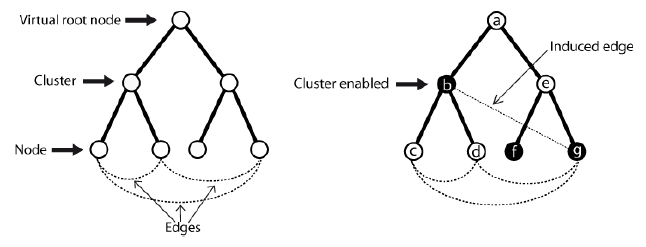
\includegraphics[width=10cm,keepaspectratio=true]{res/hierarchy.png}
  \caption{Graph tree with a virtual edge from a cluster to a leaf}
  \end{center}
\end{figure}

\paragraph{}
Two ways are available:
\begin{enumerate}
 \item Nodes can simply host other nodes and so on.
 \item Each node refers to a parent node id with the XML-attribute \begin{footnotesize}pid\end{footnotesize}.
\end{enumerate}

The first style is preferred when the structure written is previously ordered. Sequential reading of this kind of GEXF is safe because no node reference is used. But in the case your program can't provide this, the second way allows writing (and then reading) nodes randomly, but linear reading is at your own risks.

\subsection{Sequential-safe Reading}

\lstset{ style=gexf }
\begin{lstlisting}[caption={First way},label=hierarchy1]
    <graph mode="static" defaultedgetype="directed">
        <nodes>
          <node id="a" label="Kevin Bacon">
            <nodes>
              <node id="b" label="God">
                <nodes>
                  <node id="c" label="human1"/>
                  <node id="d" label="human2"/>
                </nodes>
              </node>
              <node id="e" label="Me">
                <nodes>
                  <node id="f" label="frog1"/>
                  <node id="g" label="frog2"/>
                </nodes>
              </node>
            </nodes>
          </node>
        </nodes>
        <edges>
            <edge source="b" target="e" />
            <edge source="c" target="d" />
            <edge source="g" target="b" />
            <edge source="f" target="a" />
        </edges>
    </graph>
\end{lstlisting}

Note that edges are not necessarily written at the end:
\lstset{ style=gexf }
\begin{lstlisting}[caption={First way with edges inside clusters},label=hierarchy11]
    <graph mode="static" defaultedgetype="directed">
        <nodes>
          <node id="a" label="Kevin Bacon">
            <nodes>
              <node id="b" label="God">
                <nodes>
                  <node id="c" label="human1"/>
                  <node id="d" label="human2"/>
                </nodes>
                <edges>
                  <edge source="c" target="d" />
                </edges>
              </node>
              <node id="e" label="Me">
                <nodes>
                  <node id="f" label="frog1"/>
                  <node id="g" label="frog2"/>
                </nodes>
              </node>
            </nodes>
            <edges>
              <edge source="b" target="e" />
              <edge source="f" target="a" />
              <edge source="g" target="b" />
            </edges>
          </node>
        </nodes>
        <edges />
    </graph>
\end{lstlisting}

\subsection{Random Writing}

If you can't structure your graph topology before writing a GEXF file, you may use the second style. Nodes sent to Gephi from a live data source, i.e. a web crawler, are written like this. Note that edges are always written randomly.

\lstset{ style=gexf }
\begin{lstlisting}[caption={Second way},label=hierarchy2]
<nodes>
  <node id="a" label="Kevin Bacon" />
  <node id="b" label="God" pid="a" />
  <node id="c" label="human1" pid="b" />
  <node id="d" label="human2" pid="b" />
  <node id="e" label="Me" pid="a" />
  <node id="f" label="frog1" pid="e" />
  <node id="g" label="frog2" pid="e" />
</nodes>
\end{lstlisting}

With using \begin{footnotesize}pid\end{footnotesize}, node order doesn't matter. An implementation should manage the case when a node reference (pid) is used before the node declaration. This listings could also be:

\lstset{ style=gexf }
\begin{lstlisting}[caption={Second way randomized},label=hierarchy22]
<nodes>
  <node id="g" label="frog2" pid="e" />
  <node id="a" label="Kevin Bacon" />
  <node id="c" label="human1" pid="b" />
  <node id="b" label="God" pid="a" />
  <node id="e" label="Me" pid="a" />
  <node id="d" label="human2" pid="b" />
  <node id="f" label="frog1" pid="e" />
</nodes>
\end{lstlisting}


\section{Advanced Concepts II: Phylogeny structure} \label{phylogeny}

Multiple parents can be addressed with the following syntax, where a and b are c's parents:
\lstset{ style=gexf }
\begin{lstlisting}[caption={Multiple parents},label=phylogeny1]
<nodes>
  <node id="a" label="cheese">
  <node id="b" label="cherry">
  <node id="c" label="cake">
    <parents>
      <parent for="a" />
      <parent for="b" />
    </parents>
  </node>
</nodes>
\end{lstlisting}

\section{Advanced Concepts III: Dynamics} \label{dynamics}

As networks dynamics is a growing topic of research, GEXF format includes extensive time support. Enable it by setting the \begin{footnotesize}mode\end{footnotesize} attribute of the graph to \textit{dynamic}.

\lstset{ style=gexf }
\begin{lstlisting}[caption={Dynamic Enabled!},label=dynamicEnabled]
<graph mode="dynamic">
  ...
</graph>
\end{lstlisting}

Both network topology and attributes can be dynamic. Time values in GEXF can be represented either via numbers or date or date plus time. In addition, the time representation can either use timestamps or intervals. We'll go into more details later. In the example below is uses the date time format and the default interval time representation.

\subsection{Example}

\lstset{ style=gexf }
\begin{lstlisting}[caption={A (small) Dynamic Web Graph with date format},label=dynwebgraph]
<?xml version="1.0" encoding="UTF-8"?>
<gexf xmlns="http://gexf.net/1.3.1"
       xmlns:xsi="http://www.w3.org/2001/XMLSchema-instance"
       xsi:schemaLocation="http://gexf.net/1.3.1
                             http://gexf.net/1.3.1/gexf.xsd"
      version="1.3">
  <graph mode="dynamic" defaultedgetype="directed" timeformat="date">
    <attributes class="node" mode="static">
      <attribute id="0" title="url" type="string"/>
      <attribute id="1" title="frog" type="boolean">
        <default>true</default>
      </attribute>
    </attributes>
    <attributes class="node" mode="dynamic">
      <attribute id="2" title="indegree" type="float"/>
    </attributes>
    <nodes>
      <node id="0" label="Gephi" start="2009-03-01">
        <attvalues>
          <attvalue for="0" value="http://gephi.org"/>
          <attvalue for="2" value="1"/>
        </attvalues>
      </node>
      <node id="1" label="Webatlas">
        <attvalues>
          <attvalue for="0" value="http://webatlas.fr"/>
          <attvalue for="2" value="1" end="2009-03-01"/>
          <attvalue for="2" value="2" start="2009-03-01" end="2009-03-10"/>
          <attvalue for="2" value="1" start="2009-03-11"/>
        </attvalues>
      </node>
      <node id="2" label="RTGI" end="2009-03-10">
        <attvalues>
          <attvalue for="0" value="http://rtgi.fr"/>
          <attvalue for="2" value="0" end="2009-03-01"/>
          <attvalue for="2" value="1" start="2009-03-01"/>
        </attvalues>
      </node>
      <node id="3" label="BarabasiLab">
        <attvalues>
          <attvalue for="0" value="http://barabasilab.com"/>
          <attvalue for="1" value="false"/>
          <attvalue for="2" value="0" end="2009-03-01"/>
          <attvalue for="2" value="1" start="2009-03-01"/>
        </attvalues>
      </node>
    </nodes>
    <edges>
      <edge source="0" target="1" start="2009-03-01"/>
      <edge source="0" target="2"
             start="2009-03-01" end="2009-03-10"/>
      <edge source="1" target="0" start="2009-03-01"/>
      <edge source="2" target="1" end="2009-03-10"/>
      <edge source="0" target="3" start="2009-03-01"/>
    </edges>
  </graph>
</gexf>
\end{lstlisting}

\subsection{Time representation}

GEXF aims to offer equivalent features for both time representations: \textit{timestamp} and \textit{intervals}. Timestamps are unique points in time while intervals can represent a duration and may include infinity as one of its bounds.

\paragraph{}
The two time representations can't however be mixed in GEXF and should be defined and consistent throughout the graph.

\lstset{ style=gexf }
\begin{lstlisting}[caption={Timestamp Time Representation}]
<graph mode="dynamic" timerepresentation="timestamp">
...
</graph>
\end{lstlisting}

The default time representation is \begin{footnotesize}interval\end{footnotesize} to be backward compatible with previous GEXF versions as the timestamp representation is only introduced in 1.3.

\lstset{ style=gexf }
\begin{lstlisting}[caption={Interval Time Representation}]
<graph mode="dynamic" timerepresentation="interval">
...
</graph>
\end{lstlisting}

Note that intervals are always defined with a pair of attributes \textit{start} and \textit{end}. Omitting one of the two translates into an infinity bound. For instance, \begin{footnotesize}node id="0" label="Foo" start="2005"\end{footnotesize} translates into a \begin{footnotesize}[2005, +INF]\end{footnotesize} interval for the node.

\subsection{Time format}

Time in GEXF can be encoded in two ways: via numbers or via dates and times. This is controlled via the \begin{footnotesize}timeformat\end{footnotesize} attribute set on the graph element.

\paragraph{}
As a number, it is an \textit{integer} or a \textit{double}. As a date, it is encoded as an international standard \textit{date} (yyyy-mm-dd) or a \textit{dateTime} defined by the corresponding \href{http://www.w3.org/TR/xmlschema-2/#dateTime}{XSD Datatype}. If omitted, the default type is \textit{double}.

\lstset{ style=gexf }
\begin{lstlisting}[caption={Double format}]
<graph mode="dynamic" timeformat="double">
  <nodes>
    <node id="0" label="Gephi" start="1.0" />
    <node id="1" label="Gexf" start="2.0" end="3.0" />
    ...
  </nodes>
</graph>
\end{lstlisting}

\lstset{ style=gexf }
\begin{lstlisting}[caption={Date format}]
<graph mode="dynamic" timeformat="date">
  <nodes>
    <node id="0" label="Gephi" start="2003-01-01" />
    <node id="1" label="Gexf" start="2003-01-01" end="2004-01-01" />
    ...
  </nodes>
</graph>
\end{lstlisting}

\lstset{ style=gexf }
\begin{lstlisting}[caption={Datetime format (also with timezone)}]
<graph mode="dynamic" timeformat="dateTime">
  <nodes>
    <node id="0" label="Gephi" start="2012-09-12T15:04:01" />
    <!-- With timezone -->
    <node id="1" label="Gexf" start="2012-11-04T11:00:01+03:00"
      end="2012-15-04T11:00:01+03:00" />
    ...
  </nodes>
</graph>
\end{lstlisting}

The timezone can also set globally for the entire graph via the \begin{footnotesize}timezone\end{footnotesize} graph attribute.

\lstset{ style=gexf }
\begin{lstlisting}[caption={Global timezone setting}]
<graph mode="dynamic" timeformat="dateTime" timezone="America/Los_Angeles">
...
</graph>
\end{lstlisting}

\subsection{Dynamic Topology}

Graph nodes and edges can exist at various points in time. Existence in time can be represented in different ways.

\subsubsection{Unique interval or timestamp}

The simplest way is by setting a pair of \begin{footnotesize}start\end{footnotesize} and \begin{footnotesize}end\end{footnotesize} for the interval time representation and \begin{footnotesize}timestamp\end{footnotesize} for the timestamp time representation.

\lstset{ style=gexf }
\begin{lstlisting}[caption={Node Scope Example with Intervals}]
<graph mode="dynamic" timerepresentation="interval">
  <nodes>
    <node id="0" label="Hello" start="2019-01-01" end="2019-02-01" />
    <node id="1" label="World" start="2019-01-15" end="2019-03-20" />
    ...
  </nodes>
</graph>
\end{lstlisting}

\lstset{ style=gexf }
\begin{lstlisting}[caption={Node Scope Example with Timestamps}]
<graph mode="dynamic" timerepresentation="timestamp">
  <nodes>
    <node id="0" label="Hello" timestamp="2019-01-01" />
    <node id="1" label="World" timestamp="2019-03-20" />
    ...
  </nodes>
</graph>
\end{lstlisting}

Each edge must declare time limits inside the join scope of its \begin{footnotesize}source\end{footnotesize} and \begin{footnotesize}target\end{footnotesize} nodes:
\begin{itemize}
 \item edge.start $\le$ (source.start and target.start)
 \item edge.end   $\ge$ (source.end   and target.end)
\end{itemize}

\lstset{ style=gexf }
\begin{lstlisting}[caption={Edge Scope Example}]
<nodes>
  <node id="0" label="Hello" start="2009-01-01" end="2009-02-01" />
  <node id="1" label="World" start="2009-01-15" end="2009-03-20" />
  ...
</nodes>
<edges>
  <edge source="0" target="1" start="2009-01-20" end="2009-02-01"/>
</edges>
\end{lstlisting}

Important: \begin{footnotesize}start\end{footnotesize} and \begin{footnotesize}end\end{footnotesize} values are inclusive, i.e. the following line is allowed:

\lstset{ style=gexf }
\begin{lstlisting}[caption={Smallest time scope}]
<edge source="0" target="1" start="2009-01-20" end="2009-01-20"/>
\end{lstlisting}

And of course the \begin{footnotesize}end\end{footnotesize} value must be equal or later than the \begin{footnotesize}start\end{footnotesize} value.

\subsubsection{Spells}

If a node or an edge exists at multiple timestamps or intervals, we use the concept of spells. Use the xml-element \begin{footnotesize}spells\end{footnotesize} for topology like this:

\lstset{ style=gexf }
\begin{lstlisting}[caption={Node with multiple spells (Intervals)}]
<graph mode="dynamic" timeformat="date" timerepresentation="interval">
  <nodes>
    <node id="0" label="Hello">
      <spells>
        <spell start="2009-01-01" end="2009-01-15" />
        <spell start="2009-01-30" end="2009-02-01" />
      </spells>
    </node>
    ...
  </nodes>
</graph>
\end{lstlisting}

If no \begin{footnotesize}start\end{footnotesize} is provided, the spell begins with the network. If no \begin{footnotesize}end\end{footnotesize} is provided, the spell ends with the network. If two spells are covering a same period of time, parsers should consider them as a unique spell.

\lstset{ style=gexf }
\begin{lstlisting}[caption={Node with multiple spells (Timestamps)}]
<graph mode="dynamic" timeformat="date" timerepresentation="timestamp">
  <nodes>
    <node id="0" label="Hello">
      <spells>
        <spell timestamp="2009-01-15" />
        <spell timestamp="2009-02-01" />
      </spells>
    </node>
    ...
  </nodes>
</graph>
\end{lstlisting}

If spells are provided, only their content are taken into account and other time attributes on the element like \begin{footnotesize}timestamp\end{footnotesize} will be ignored.

\paragraph{}
Important: Intervals can't overlap for an element.

\lstset{ style=gexf }
\begin{lstlisting}[caption={Overlapping intervals (not allowed)}]
<graph mode="dynamic" timeformat="date" timerepresentation="interval">
  <nodes>
    <node id="0" label="Hello">
      <spells>
        <spell start="2009-01-01" end="2009-01-15" />
        <spell start="2009-01-05" end="2009-02-01" />
      </spells>
    </node>
  ...
  </nodes>
</graph>
\end{lstlisting}

\subsubsection{Alternative to spells}

For a more compact spell representation, GEXF also offers \begin{footnotesize}timestamps\end{footnotesize} and \begin{footnotesize}intervals\end{footnotesize} attributes as lists. It's however less safe as it relies more heavily on the parser. Make sure to check the following examples.

\lstset{ style=gexf }
\begin{lstlisting}[caption={Timestamp list (Date)}]
<graph mode="dynamic" timerepresentation="timestamp" timeformat="date">>
  <nodes>
    <node id="0" label="Hello" timestamps="<[2019-03-20, 2019-03-21]>" />
    ...
  </nodes>
</graph>
\end{lstlisting}

\lstset{ style=gexf }
\begin{lstlisting}[caption={Timestamp list (Double)}]
<graph mode="dynamic" timerepresentation="timestamp" timeformat="double">>
  <nodes>
    <node id="0" label="Hello" timestamps="<[1, 2, 21.0, 124.0]>" />
    ...
  </nodes>
</graph>
\end{lstlisting}

\lstset{ style=gexf }
\begin{lstlisting}[caption={Interval list (Double)}]
<graph mode="dynamic" timerepresentation="timestamp" timeformat="double">>
  <nodes>
    <node id="0" label="Hello" intervals="<[4.0, 14.0]; [21.0, 124.0]>" />
    ...
  </nodes>
</graph>
\end{lstlisting}

Note that the separator between intervals is a semi-colon as the comma is reserved for the interval itself.

\paragraph{}
About the weight: dynamic weight can be used with the reserved \textit{title} "weight" in attributes. In dynamic mode, the static XML-attribute \textit{weight} should be ignored if the dynamic one is provided.

\subsection{Dynamic Data}

Node and edges data can take different values over time. Attributes must be declared as dynamic, allowing values to exist for a given time.

\subsubsection{Declaring Dynamic Attributes}

\lstset{ style=gexf }
\begin{lstlisting}[caption={Indegree may change over time}]
<gexf ...>
  ...
  <graph mode="dynamic" defaultedgetype="directed">
    <attributes class="node">
      <attribute id="2" title="indegree" type="float"/>
      ...
    </attributes>
    ...
  </graph>
</gexf>
\end{lstlisting}

\subsubsection{Defining Dynamic Values}

Attvalues have their scopes limited by the xml-attributes \begin{footnotesize}start\end{footnotesize} and \begin{footnotesize}end\end{footnotesize}.

\lstset{ style=gexf }
\begin{lstlisting}[caption={Data value changing over time}]
<node id="3" label="BarabasiLab">
  <attvalues>
    <attvalue for="2" value="0" start="2009-01-01" end="2009-03-01"/>
    <attvalue for="2" value="1" start="2009-03-02" end="2009-03-10"/>
  </attvalues>
</node>
\end{lstlisting}

\lstset{ style=gexf }
\begin{lstlisting}[caption={Using timestamp representation}]
<node id="3" label="BarabasiLab">
  <attvalues>
    <attvalue for="2" value="15.0" timestamp="2000" />
    <attvalue for="2" value="20.0" timestamp="2005" />
    <attvalue for="2" value="25.0" timestamp="2010" />
  </attvalues>
</node>
\end{lstlisting}

\subsubsection{Dynamic Values and Spells}

If an \begin{footnotesize}attvalue\end{footnotesize} is covering a period out of any spell, this period should be ignored by parsers. In the following example, the day 2009-01-03 is ignored:

\lstset{ style=gexf }
\begin{lstlisting}[caption={Spells and attvalues}]
<gexf ...>
  ...
  <graph mode="dynamic">
    <node id="0" label="Hello">
      <attvalues>
        <attvalue for="0" value="1" start="2009-01-01" end="2009-01-05"/>
      </attvalues>
      <spells>
        <spell start="2009-01-01" end="2009-01-02" />
        <spell start="2009-01-04" end="2009-01-05" />
      </spells>
    </node>
    ...
  </graph>
</gexf>
\end{lstlisting}

\section{Advanced Concepts IV: Extending GEXF} \label{extendgexf}

GEXF is designed to be easily extensible. Additional namespaces are defined by an XML Schema. The default namespace is always the gexf namespace. Gephi team actually provides a module for storing visualization data called \textit{viz}.

\subsection{VIZ module} \label{viz}

Using the visualization module must be declared by adding the XML Attribute \begin{footnotesize}xmlns:viz="http://gexf.net/1.3.1/viz"\end{footnotesize} to the document namespaces. The \begin{footnotesize}xsi:schemaLocation\end{footnotesize} attribute includes the XML-Schema declaration of the VIZ module. The RelaxNG Compact specification is available in \href{http://gexf.net/1.3.1/viz.rnc}{viz.rnc}, and independent XSD declaration in \href{http://gexf.net/1.3.1/viz.xsd}{viz.xsd}.

\paragraph{}
Color, position, size and shape are stored as attributes.

\subsubsection{Viz attributes}

\paragraph{Node Example}

The following gexf contains a node having a color, a position, a shape and a specified size.

\lstset{ style=gexf }
\begin{lstlisting}[caption={VIZ Attributes},label=vizattr]
<gexf xmlns="http://gexf.net/1.3.1"
      xmlns:viz="http://gexf.net/1.3.1/viz">
...
  <node ... >
    <viz:color r="239" g="173" b="66" a="0.5"/>
    <viz:position x="15.783598" y="40.109245" z="0.0"/>
    <viz:size value="2.0375757"/>
    <viz:shape value="disc"/>
  </node>
...
</gexf>
\end{lstlisting}

\paragraph{Edge Example}

The following gexf contains an edge having a color, a thickness and a shape.

\lstset{ style=gexf }
\begin{lstlisting}[caption={VIZ Attributes},label=vizattr]
<gexf xmlns="http://gexf.net/1.3.1"
      xmlns:viz="http://gexf.net/1.3.1/viz">
...
  <edge ... >
    <viz:color r="157" g="213" b="78"/>
    <viz:thickness value="5.124"/>
    <viz:shape value="solid"/>
  </edge>
...
</gexf>
\end{lstlisting}

\paragraph{Color}

Colors are defined by the \href{http://en.wikipedia.org/wiki/RGBA}{RGBA color model}. Each XML-attribute value \begin{footnotesize}r\end{footnotesize}, \begin{footnotesize}g\end{footnotesize} or \begin{footnotesize}b\end{footnotesize} is hence an integer from 0 to 255, and the alpha value \begin{footnotesize}a\end{footnotesize} is a float from 0.0 to 1.0.

\lstset{ style=gexf }
\begin{lstlisting}[caption={VIZ Color Declaration},label=vizcolor]
<viz:color r="239" g="173" b="66" a="0.5"/>
\end{lstlisting}

Colors can alternatively be defined with a unique \begin{footnotesize}hex\end{footnotesize} attribute. It can still be combined with the alpha parameter

\lstset{ style=gexf }
\begin{lstlisting}[caption={Color Hex Attribute},label=vizhex]
<viz:color hex="#FF7700" alpha="0.5"/>
\end{lstlisting}

\paragraph{Position}

Space positions are set in three dimensions called \begin{footnotesize}x\end{footnotesize}, \begin{footnotesize}y\end{footnotesize} and \begin{footnotesize}z\end{footnotesize}. Note that Gephi associates \begin{footnotesize}z\end{footnotesize} (optional) as the height, and most of layout algorithms only use \begin{footnotesize}x\end{footnotesize} and \begin{footnotesize}y\end{footnotesize}. They are floats.

\lstset{ style=gexf }
\begin{lstlisting}[caption={VIZ Position Declaration},label=vizposition]
<viz:position x="15.783598" y="40.109245" z="0.0"/>
\end{lstlisting}

\paragraph{Size}

Node size is a scale. It is set to \textit{1.0} by default and is a non-negative float. Network viz softwares assume that an object representing a node of size \textit{2.0} is twice bigger as one of \textit{1.0}.

\lstset{ style=gexf }
\begin{lstlisting}[caption={VIZ Size Declaration},label=vizsize]
<viz:size value="2.0375757"/>
\end{lstlisting}

\paragraph{Thickness}

Edge thickness is a scale. It is set to \textit{1.0} by default and is a non-negative float. Network viz softwares assume that an object representing an edge of thickness \textit{2.0} is twice bigger as one of \textit{1.0}.

\lstset{ style=gexf }
\begin{lstlisting}[caption={VIZ Thickness Declaration},label=vizthickness]
<viz:thickness value="2.0375757"/>
\end{lstlisting}

\paragraph{Node Shape}

Default node is shaped as a disc. Four shapes are proposed: \textit{disc}, \textit{square}, \textit{triangle} and \textit{diamond}. Images require an additional xml-attribute to set their location: \begin{footnotesize}uri\end{footnotesize}.

\lstset{ style=gexf }
\begin{lstlisting}[caption={Image Declaration},label=vizimage]
<viz:shape value="image" uri="http://my.image.us/blah.jpg"/>
\end{lstlisting}

\paragraph{Edge Shape}

Default edge is shaped as solid. Four shapes are proposed: \textit{solid}, \textit{dotted}, \textit{dashed} and \textit{double}.

\subsubsection{Scale}

The nodes/edges viz attributes described in previous section are stored as static data. This means that they don't mention why the viz:color has been set to this particular value. It's encoded as if the color has been chosen by hand without any data logic. But very often those viz attributes are actually computed from data attributes using for instance the Partition/Ranking features in Gephi.
The scale features are meant to be able to inform Gexf consumers about the viz attributes logic in order to support legend drawing aside visualizing the graph.

Scales can be described at the graph level in the attributes element.
Plural version of viz attributes: `viz:colors`, `viz:sizes`, `viz:shapes`, `viz:positions`, `viz:thicknesses` are used to host the dynamic definitions of viz attributes.

\paragraph{}
We propose to include those into the the attribute(s) definitions in order to:
\begin{itemize}
\item Set the rule globally for the graph
\item Reuse the node/edge class attribute already set in the attributes
\item Nest the scale definition inside the corresponding attribute definition
\end{itemize}

\paragraph{}
To represent the dynamic definitions of viz attributes we need to define:
\begin{itemize}
\item which attribute to use: nested in attribute definition...
\item the scale type: quantitative, qualitative, layout...
\item the parameters: color hashmap, range, spline method...
\end{itemize}

A GEXF can host more than one for one viz parameter. For instance colors could be derived from two different node attributes type and degree. Therefore a \textit{defaultscales} element can be used to specify which scale has been used to render the colors, sizes (...) in the gexf.

The scale information are meant to be used to draw a legend. But they can also theoretically be used to generate the according viz parameters.
Yet a GEXF file can contain both viz attributes at the node/edge levels (local) and a viz scale at the graph level (global).
The local viz attributes must take over global definition when rendering visually a GEXF.
To ensure the best GEXF compatibility among existing consumers we recommend to set both local and global systematically.

\paragraph{Scale Example}

The following gexf contains an gexf attributes section which embed colors, sizes and positions legend information.

\lstset{ style=gexf }
\begin{lstlisting}[caption={VIZ Scales},label=vizscales]
<gexf xmlns="http://gexf.net/1.3.1"
      xmlns:viz="http://gexf.net/1.3.1/viz">
...
  <attributes class="node" mode="static">
    <attribute id="type" title="type" type="string">
      <viz:colors scale="qualitative">
        <viz:color forvalue="person" hex="#FF0000"/>
        <viz:color forvalue="city" hex="#00FF00"/>
      </viz:colors>
    </attribute>
    <attribute id="degree" title="Degree" type="integer">
      <default>0</default>
      <viz:sizes scale="quantitative" scalelabel="square-root">
        <viz:scalepoint forratio="0" factor="0" />
        <viz:scalepoint forratio="0.1" factor="0.316227766"/>
        <viz:scalepoint forratio="0.2" factor="0.447213595"/>
        <viz:scalepoint forratio="0.3" factor="0.547722558"/>
        <viz:scalepoint forratio="0.4" factor="0.632455532"/>
        <viz:scalepoint forratio="0.5" factor="0.707106781"/>
        <viz:scalepoint forratio="0.6" factor="0.774596669"/>
        <viz:scalepoint forratio="0.7" factor="0.836660027"/>
        <viz:scalepoint forratio="0.8" factor="0.894427191"/>
        <viz:scalepoint forratio="0.9" factor="0.948683298"/>
        <viz:scalepoint forratio="1.0" factor="1"/>
        <viz:range min="1" max="10" default="1" />
      </viz:sizes>
    </attribute>
    <viz:defaultscales  colors="type" sizes="degree" />
    <viz:positions layoutalgorithm="forceatlas2" 
      referenceURL="https://journals.plos.org/plosone/article?id=10.1371/journal.pone.0098679">
      <viz:param name="scale" type="integer" value="10"/>
      <viz:param name="stronger gravity" type="boolean" value="true"/>
    </viz:positions>
  </attributes>
  <attributes class="edge" mode="static">
    <attribute id="type" title="type" type="string">
      <viz:colors scale="qualitative">
        <viz:color forvalue="lives in" hex="#112345"/>
        <viz:color forvalue="works with" hex="#654523"/>
      </viz:colors>
    </attribute>
    <viz:defaultscales colors="type"/>
  </attributes>
...
</gexf>
\end{lstlisting}

\paragraph{Qualitative color scale} The \textit{viz:colors} describe a \textit{qualitative} scale which uses the \textit{modularityclass} node attribute to define the node's \textit{viz:color} attribute.
To do so the \textit{viz:colors} element contains a color palette attributing a color for each value. A \textit{viz:colordefault} can be used to handle null or not listed values.

\lstset{ style=gexf }
\begin{lstlisting}[caption={Qualitative color scale},label=vizscalecolorquali]
<attributes class="node" mode="static">
    <attribute id="modularityclass" title="Modularity Class" type="integer">
        <default>0</default>
        <viz:colors scale="qualitative">
            <viz:color forvalue="1" r="168" g="168" b="29"/>
            <viz:color forvalue="2" r="204" g="16" b="210"/>
            <viz:color forvalue="3" r="156" g="54" b="54"/>
            <viz:color forvalue="4" r="200" g="180" b="92"/>
            <viz:colordefault r="1" g="1" b="1"/>
        </viz:colors>
    </attribute>
</attributes>
\end{lstlisting}

\paragraph{Quantitative color scale} The \textit{viz:colors} can also describe a \textit{quantitative} scale which uses the \textit{degree} node attribute to define the node's \textit{viz:color} attribute.
To do so the \textit{viz:colors} element contains a color gradient definition defining color points on a 0-1 value scale. The \textit{scalelabel} attribute is useful to give more textual description of the scale logic.

\lstset{ style=gexf }
\begin{lstlisting}[caption={Quantitative color scale},label=vizscalecolorquanti]
  <attributes class="node" mode="static">
  <attribute id="degree" title="Degree" type="integer">
      <default>0</default>
      <viz:colors scale="quantitative" scalelabel="greenish gradient">
          <viz:color forratio="0" hex="#EDF8FB"/>
          <viz:color forratio="0.5" hex="#66C2A4"/>
          <viz:color forratio="1" r="0" g="109" b="44"/>
      </viz:colors>
  </attribute>
</attributes>
\end{lstlisting}

\paragraph{Concurrent color scales} There can be more than one \textit{viz:colors} in the node attributes. To inform which scale were used to compute the colors encoded in the GEXF, a \textit{viz:defaultscales} element nested inside \textit{attributes} indicates which is the default scale to be used.

\lstset{ style=gexf }
\begin{lstlisting}[caption={Quantitative color scale},label=vizscalecolorquanti]
  <attributes class="node" mode="static">
    <attribute id="modularityclass" title="Modularity Class" type="integer">
      <default>0</default>
      <viz:colors scale="qualitative">
          <viz:color forvalue="1" r="168" g="168" b="29"/>
          <viz:color forvalue="2" r="204" g="16" b="210"/>
          <viz:color forvalue="3" r="156" g="54" b="54"/>
          <viz:color forvalue="4" r="200" g="180" b="92"/>
          <viz:colordefault r="1" g="1" b="1"/>
      </viz:colors>
    </attribute>
    <attribute id="degree" title="Degree" type="integer">
        <default>0</default>
        <viz:colors scale="quantitative" scalelabel="greenish gradient">
            <viz:color forratio="0" hex="#EDF8FB"/>
            <viz:color forratio="0.5" hex="#66C2A4"/>
            <viz:color forratio="1" r="0" g="109" b="44"/>
        </viz:colors>
    </attribute>
    <viz:defaultscales colors="type" />
</attributes>
\end{lstlisting}

\paragraph{Quantitative size scale} For \textit{quantitative} scale, \textit{viz:scalepoint} elements can be used to define an transformation function to adapt node attributes values to the viz (size here) parameters. The function is expressed as a set of points which represents a [0-1] to [0-1] curve. Here the \textit{scalelabel} indicates that this set of points actually represent a square-root function. Although a set of discreet point is not as precise as a real function expression it has been preferred as function expression would have mean choosing a syntax and is more flexible than a finite set of function name.

\lstset{ style=gexf }
\begin{lstlisting}[caption={Quantitative size scale},label=vizscalesizequanti]
<attributes class="node" mode="static">
    <attribute id="degree" title="Degree" type="integer">
        <default>0</default>
        <viz:sizes scale="quantitative" scalelabel="square-root">
            <viz:scalepoint forratio="0" factor="0" ></viz:scalepoint>
            <viz:scalepoint forratio="0.1" factor="0.316227766" ></viz:scalepoint>
            <viz:scalepoint forratio="0.2" factor="0.447213595"></viz:scalepoint>
            <viz:scalepoint forratio="0.3" factor="0.547722558"></viz:scalepoint>
            <viz:scalepoint forratio="0.4" factor="0.632455532"></viz:scalepoint>
            <viz:scalepoint forratio="0.5" factor="0.707106781"></viz:scalepoint>
            <viz:scalepoint forratio="0.6" factor="0.774596669"></viz:scalepoint>
            <viz:scalepoint forratio="0.7" factor="0.836660027"></viz:scalepoint>
            <viz:scalepoint forratio="0.8" factor="0.894427191"></viz:scalepoint>
            <viz:scalepoint forratio="0.9" factor="0.948683298"></viz:scalepoint>
            <viz:scalepoint forratio="1" factor="1"></viz:scalepoint>
            <viz:range min="1" max="10" default="1" />
        </viz:sizes>
    </attribute>
</attributes>
\end{lstlisting}

\paragraph{Positions layout} Nodes layouts are algorithms which are used to calculate (x,y) node positions. As they usually are not bind on one specific attribute the \textit{vis:positions} element is placed in the \textit{attributes} element. It documents which algorithm(s) has been used with an optional \textit{referenceURL}. The \textit{vis:layout} element contains a list of parameters which were used. Each \textit{vis:layout} must have a \textit{step} attribute which indicates in which order the layouts were applied.

\lstset{ style=gexf }
\begin{lstlisting}[caption={Positions layout},label=vizpositionlayout]
<attributes class="node" mode="static">
    <attribute id="degree" title="Degree" type="integer">
        <default>0</default>
    </attribute>
    <viz:positions> 
      <viz:layout algorithm="forceatlas2" referenceURL="https://journals.plos.org/plosone/article?id=10.1371/journal.pone.0098679" step="1">
        <viz:param name="scale" type="integer" value="10"/>
        <viz:param name="stronger gravity" type="boolean" value="true"/>
      </viz:layout>
      <viz:layout algorithm="nooverlap" step="2">
        <viz:param name="speed" type="integer" value="3"/>
        <viz:param name="ratio" type="float" value="1.2"/>
        <viz:param name="margin" type="float" value="5.0"/>
      </viz:layout>  
    </viz:positions>
</attributes>
\end{lstlisting}

\section{Advices: Parser optimization} \label{advices}

This section provides some good tips to write parser-friendly files.
\begin{itemize}
 \item Always place the edges after the nodes, as it is mandatory since version 1.2. Some parsers, depending on their implementation, may reject an edge if its linked nodes haven't been declared before, due to conceptual or data integrity reason.
 \item Use the \textit{count} XML-attribute in \textit{nodes} and \textit{edges} declaration: the parser will know how much memory it should allocate, and will speed up the file reading. Note that count only refers to direct children, not the whole sub-graph!
 \item Prefer \textit{liststring} to \textit{string} attributes if you can. A smart parser will store the strings in one place, and just set pointers to them from the related nodes/edges.
 \item Identifiers may be interpreted as integers if you only use numbers. We encourage this practice, as an integer takes much less size in memory than an equivalent string. Tell the parser to optimize IDs storage by filling the optional graph XML-attribute called \textit{idtype} with \textit{string}, \textit{integer} or \textit{long}.
\end{itemize}

\section{Web Services} \label{ws}

The content-type for serving GEXF files via HTTP/REST is \textit{application/gexf+xml}.

\section{Resources} \label{resources}

Specifications are available on GitHub at \href{https://github.com/gephi/gexf/}{https://github.com/gephi/gexf/}. Contributions and feedback are welcome.

\paragraph{}
The website \href{https://gexf.net}{https://gexf.net} contains additional examples and links to popular libraries capable of reading and writing the format.

\section{Changelog} \label{changelog}

Note that we used to use "draft" in certain version (e.g "1.2draft") up until 1.3 when we decided to simply use full versions numbers.

\paragraph{}
The GEXF specification history:

\subsection*{Version 1.3.1}

\begin{itemize}
\item Added a title element in graph
\item Extend `viz` module to support legend drawing
\end{itemize}

\subsection*{Version 1.3}

\begin{itemize}
\item Add `kind` attribute on `edge` to support multi-graph (i.e. parallel edges)
\item The edge `weight` is now a `double` instead of a `float`
\item The edge `id` is now optional
\item Add `xsd:long`as possible `idtype` on `\<graph\>`
\item Add new attribute types `bigdecimal`, `biginteger`, `char`, `short` and `byte`
\item Add new list attributes like `listboolean` or `listinteger` for each atomic type
\item Dynamics
\begin{itemize}
\item Add a `timezone` attribute on `\<graph\>` to use as a timezone in case it's omitted in the element timestamps
\item Open intervals attributes `startopen` and `endopen` are removed. Use regular inclusive `start` and `end` instead
\item Remove `start` and `end` attributes on `\<attributes\>` as it was redundant with `\<graph\>` attributes
\item Timestamp support
\begin{itemize}
\item Add the ability to represent time with single timestamps instead of intervals. We want feature parity between the two time representations but note they can't be mixed.
\item Add a `timerepresentation` enum in `\<graph\>` with either `interval` (default) or `timestamp` to configure the way the time is represented
\item Add `timestamp` attribute to `\<node\>`, `\<edge\>`, `\<spell\>` and `\<attvalue\>` to support this new time representation
\end{itemize}
\item Alternative to spell elements
\begin{itemize}
\item Add a `timestamps` attribute to `\<node\>` and `\<edge\>` to represent a list of timestamps without having to use spells
\item Similarly, add a `intervals` attribute to `\<node\>` and `\<edge\>`
\end{itemize}
\item New slice mode
\begin{itemize}
\item The optional `mode` attribute on `\<graph\>` now has an additional `slice` value, in addition of `static` and `dynamic`. With slice, the expectation is that the `\<graph\>` also has either a `timestamp` or `start` / `end` intervals.
\item Add a `timestamp` attribute on `\<graph\>` to characterise the slice this graph represent
\item Change the meaning of the `start` and `end` attributes on `\<graph\>` to either characterise the slide instead of the time bounds, which should rather be inferred
\end{itemize}
\end{itemize}
\item Viz
\begin{itemize}
\item Add `hex` attribute on `\<color\>` so it can support values like `#FF00FF`
\item The `z` position is no longer required
\item Dynamic attributes like `start`, `end` or child elements `\<spells\>` are no longer supported for viz attributes. To represent viz attributes over time, an alternative is to create multiple graphs each representing a slice.
\end{itemize}
\end{itemize}

\subsection*{Version 1.2}

\begin{itemize}
\item The node and edge `label` attribute are now optional
\item \<meta\> should be placed before \<graph\>
\item Dynamics
\begin{itemize}
\item Rename the `timetype` attribute to `timeformat`. This attribute is set on `\<graph\>` to specify how time information is encoded, either like a date or like a double
\item The `timeformat` is currently either `float` or `date` and default value is `date`. The `float` type is replaced by `double`, and is now the default value
\item Added `timeformat` types `integer` and `dateTime`. DateTime is equivalent to timestamps
\item Add open intervals (non-inclusive): `startopen` and `endopen` attributes
\item `\<slices\>` and `\<slice\>` are renamed `\<spells\>` and `\<spell\>` respectively because slices are a different concept as remarked
\end{itemize}
\item Viz
\begin{itemize}
\item Add viz attributes support for dynamics
\item Add the alpha channel to RGB. Colors are now encoded in RGBA. It is a float from 0.0 (invisible) to 1.0 (fully visible). If omitted, the default alpha-value is 1.0 (no transparency).
\end{itemize}
\end{itemize}

\subsection*{Version 1.1}

Modules are stabilized and new ones appear: hierarchy and phylogeny.

\subsection*{Version 1.0}

First specification. Basic topology, associated data and dynamics attempt constitute the core, plus a visualization extension.

\printindex

\end{document}
